\documentclass[11pt,final,oneside]{fithesis}
\usepackage[plainpages=false, pdfpagelabels]{hyperref}
\usepackage{amssymb}
\usepackage{amsmath}
\usepackage{graphicx}
\usepackage[T1]{fontenc}
\usepackage[latin2]{inputenc}
\usepackage[slovak]{babel}

\graphicspath{{images/}}

\thesislang{sk}
\thesistitle{N\' azov diplomovej pr\' ace}
\thesissubtitle{Diplomov\' a pr\' aca}
\thesisstudent{Martin Demko}
\thesiswoman{false}
\thesisfaculty{fi}
\thesisyear{jar 2014}
\thesisadvisor{RNDr. David \v Safr\' anek, Ph.D.}

\begin{document}
\FrontMatter
\ThesisTitlePage


\begin{ThesisDeclaration}
\DeclarationText
\AdvisorName
\end{ThesisDeclaration}

\begin{ThesisThanks}
\end{ThesisThanks}

\begin{ThesisAbstract}
\end{ThesisAbstract}

\begin{ThesisKeyWords}
\end{ThesisKeyWords}

%====================================OBSAH==================================================
\MainMatter
\tableofcontents
%====================================UVOD===================================================
\chapter*{\' Uvod}


\chapter{Z\' akladn\' e pojmy}
Ne\v z za\v cneme zach\' adza\v t hlb\v sie do problematiky tejto pr\' ace a opisova\v t postupy a n\' astroje v nej pou\v zit\' e, 
je potrebn\' e vysvetli\v t na po\v ciatku nieko\v lko pojmov. Tieto sa v pr\' aci mnohokr\' at opakuj\' u a ich v\v casn\' ym uveden\' im
pred\' ideme nepochopite\v lnosti textu.

\section{LTL - Line\' arna Tempor\' alna Logika}
Tempor\' alna logika obecne je \v speci\' alna vetva logiky zaoberaj\' uca sa logickou \v strukt\' urou v\' yrokov v \v case. 
Je to formalizmus vhodn\' y pre overovanie vlastnost\' i form\' alnych dynamick\' ych syst\' emov resp. matematick\' ych modelov.

Line\' arna tempor\' alna logika (\v dalej len LTL) je najjednoduch\v sia verzia tempor\' alnej logiky, ktor\' a neumo\v z\v nuje vetvenie \v casu 
ani kvantifik\' atory.
M\^ o\v zeme ju pova\v zova\v t tie\v z za konkr\' etny v\' ypo\v ctov\' y kalkulus pracuj\' uci s tzv. formulami, definovan\' ymi nasleduj\' ucou syntaxou:
\begin{description}
\item[Atomick\' e propoz\' icie] (\v dalej len AP) \hfill
\begin{center}
$A > 0$ \\
$B \leq 5.834$ \\
$C \neq "nie"$ \\
{\it at\v d$\dots{}$}
\end{center}
\item[Logick\' e oper\' atory] \hfill
\begin{center}	%ZISTIT CI STACIA IBA -------NEGACIA, KONJUNKCIA, DISJUKCIA--------
$\neg$ , \ $\vee$\hfil\hfil\hfil\hfil\hfil - \ {\it z\' akladn\' e logick\' e oper\' atory}\\
$\wedge$ , \ $\rightarrow$ , \ $\leftrightarrow$ , \ $true$ , \ $false$ \hfil - \ {\it odvoden\' e logick\' e oper\' atory}
\end{center}
\item[Tempor\' alne oper\' atory] \hfill
\begin{center}
{\bf X} $\phi$ \ - \ ne{\bf X}t, {\it vyjadruje platnos\v t $\phi$ v \v dal\v som stave}\\
{\bf G} $\phi$ \ - \ {\bf G}lobal, {\it vyjadruje trval\' u platnos\v t $\phi$ }\\
{\bf F} $\phi$ \ - \ {\bf F}uture, {\it vyjadruje platnos\v t $\phi$ v niektorom z bud\' ucich stavov }\\
$\psi$ {\bf U} $\phi$ \ - \ {\bf U}ntil, {\it vyjadruje platnos\v t $\psi$ a\v z do kedy neza\v cne plati\v t $\phi$}\\
$\psi$ {\bf R} $\phi$ \ - \ {\bf R}elease, {\it vyjadruje platnos\v t $\phi$}\\
{\it kde $\phi$ a $\psi$ s\' u atomick\' e propoz\' icie}
\end{center}
\end{description}
Potom plat\'i nasleduj\'uce:
\begin{itemize}
\item Ak $p \in AP$, tak $p$ je formula.
\item Ak $f$ a $g$ s\'u formule, tak $\neg g$, $f \lor g$, $f \wedge g$, {\bf X} $g$, {\bf F} $g$, {\bf G} $g$, $f$ {\bf U} $g$ a $g$ {\bf R} $f$ s\'u formule.
\end{itemize}
Napriek tomu, \v ze je LTL tou najprimit\' ivnej\v sou tempor\'alnou logikou, jej prevod do B\"uchiho automatu je v najhor\v som pr\' ipade 
exponenci\' alne zlo\v zit\' y. D\^ ovod tohto prevodu bude vysvetlen\' y v kapitole \ref{model_checking}.

\section{B\"uchiho automat}	%kniha Model checking str. 121
Automat obecne je matematick\' y model stroja s kone\v cn\' ym mno\v zstvom pam\" ate spracov\' avaj\' uci vstup o nezn\' amej ve\v lkosti. 
Kv\^ oli obmedzeniu pam\" ate ho naz\' yvame kone\v cn\' ym automatom. Vstup sa naz\' yva slovo a m\^ o\v ze by\v t kone\v cn\' y aj nekone\v cn\' y.
B\" uchiho automat je potom najjednoduch\v s\' im kone\v cn\'ym automatom nad nekone\v cn\'ym slovom a preto patr\'i do skupiny {$\omega$"~au\-to\-matov}.

Form\'alne je kone\v cn\' y automat $\mathcal{A}$ p\" atica $(\Sigma, Q, \Delta, Q_0, F)$, pre ktor\' u plat\'i:
\begin{itemize}
\item $\Sigma$\ je kone\v cn\'a abeceda
\item $Q$\ je kone\v cn\'a mno\v zina stavov
\item $\Delta \subseteq Q \times \Sigma \times Q$\ je rel\' acia naz\'yvan\'a prechodov\'a funkcia
\item $Q_0 \subseteq Q$ je podmno\v zina mno\v ziny stavov, naz\' yvan\' a inici\' alne stavy
\item $F \subseteq Q$ je podmno\v zina mno\v ziny stavov, naz\'yvan\'a akceptuj\'uce stavy
\end{itemize}
Pr\'iklad jednoduch\'eho automatu je dan\'y na obr\'azku \ref{fig:buchi}.Automat nad kone\v cn\'ym slovom akceptuje toto slovo, ak po prejden\' i poslen\'eho znaku slova zodpovedaj\' uceho prechodu medzi dvoma stavami, 
je tento posledn\' y stav v mno\v zine $F$. Av\v sak automat nad nekone\v cn\' ym slovom nem\^ o\v ze nikdy prejs\v t cez posledn\' y znak. Preto tak\' yto 
automat akceptuje nekone\v cn\' e slovo len v pr\' ipade, \v ze po\v cas prech\' adzania slova je aspo\v n jeden stav nav\v st\'iven\'y nekone\v cne \v casto 
a z\'arove\v n tento stav patr\'i aj do mno\v ziny $F$.
\begin{figure}[h]
	\centering
	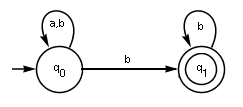
\includegraphics[width=0.6\textwidth]{Buchi01}
	\caption{Pr\'iklad jednoduch\'eho automatu}
	\label{fig:buchi}
\end{figure}



\section{Model checking}
\label{model_checking}

\section{Farebn\' y model checking}

\section{Vstupn\'y model}% ako po \v castiach multi"~afinn\'y ODE syst\'em}

\it A. \ Multi-afinn\'y ODE model\rm
\\

Vstupn\'ym modelom sa u n\'as mysl\'i model biochemick\'ych reakci\'i, ktor\'y je v na\v som po\v nat\'i bran\'y ako po \v castiach linearizovan\'y 
multi"~afinn\'y syst\'em diferenci\'alnych rovn\'ic. Ale za\v cnime od po\v ciatku a postupne sa dopracujme k tomuto v\'ysledku.

Na z\'aklade pravidla o mass~action kinetike [odkaz na wiki mass~action] je mo\v zn\'e modelova\v t \v lubovoln\'u biochemick\'u reakciu alebo dokonca 
s\'ustavu tak\'ychto reakci\'i pomocou s\'ustavy neline\'arnych oby\v cajn\'ych diferenci\'alnych rovn\'ic 
(Ordinary Differential Equations alebo ODEs) [odkaz na wiki ODE].

Uva\v zujme multi"~afinn\'y syst\'em vo forme $\dot{x} = f(x)$, kde $x = (x_1,\dots{},x_n)$ je vektor premenn\'ych a $f = (f_1,\dots{},f_n)$ \ : \ 
$\mathbb{R}^n \rightarrow \mathbb{R}^n$ je vektor multi"~afin\-n\'ych funkci\'i. Tieto funkcie s\'u vlastne polyn\'omy, v ktor\'ych je stupe\v n premenn\'ych 
$x_1,\dots{},x_n$ obmedzen\'y na hodnotu 1. Ka\v zd\'a premenn\'a $x_i$, kde $i \in \{1,\dots{},n\}$ predstavuje koncentr\'aciu \v specifickej chemickej l\'atky a je interpretovan\'a ako
{$\mathbb{R}_+ = \lbrace{}  x \in \mathbb{R}\ |\ {}x \geq 0  \rbrace$}. /*Mozno priklad*/

Z d\^ ovodu, \v ze premenn\'e m\^ ozeme vyjadri\v t len ako nez\'aporn\'e re\'alne \v cisla, je mo\v zn\'e tie\v z spojit\'y stavov\'y priestor na\v seho 
matematick\'eho syst\'emu obmedzi\v t iba na prv\'y, resp. kladn\'y kvadrant {$\mathbb{R}_+^n = \lbrace{}  x \in \mathbb{R}^n\ |\ {}x \geq 0  \rbrace$}.

Ak uva\v zujeme o premenn\'ych ako o nestabiln\'ych chemick\'ych l\'atkach, ktor\'e sami od seba degraduj\'u v \v case, m\^ o\v zme s k\v ludom obmedzi\v t 
n\'a\v s spojit\'y stavov\'y priestor $\mathcal{D}$ e\v ste viac. A s\'ice na $n$"~dimenzion\'alny obd\'l\v znik $\mathcal{D} = \prod_{i=1}^n[0,max_i] 
\subset \mathbb{R}^n$, kde $max_i$ je horn\'a hranica koncentr\'acie pre\-men\-nej $x_i$. [odkaz na hibi2010 a hibi2009]
\\

\noindent
\it B. \ Po \v castiach linearizovan\'y multi"~afinn\'y ODE model\rm
\\

Multi"~afinn\'y syst\'em diferenci\'alnych rovn\'ic dok\'a\v ze pokry\v t skoro cel\'u mass~action kinetiku s jedinou v\'ynimkou. A tou s\'u 
homodim\'ery a reakcie s nimi spojen\'e. D\^ ovodom je predch\'adzaj\'uce obmedzenie multi"~afinn\'ych funkci\'i $f_1,\dots{},f_n$ s oh\v ladom 
na stupe\v n premenn\'ych $x_1,\dots{},x_n$.

Teoreticky sme schopn\'y  pop\'isa\v t ak\' yko\v lvek biochemick\'y model pomocou pravidiel tejto kinetiky. V skuto\v cnosti, ak sa pok\'usime formulova\v t 
tieto pravidl\'a pre rozsiahly model, zist\'ime, \v ze s narastaj\'ucou ve\v lkos\v tou rastie komplexita t\'ychto pravidiel a navy\v se k \'uplnosti modelu
je potrebn\'e pozna\v t ve\v lk\'e mno\v zstvo \v co najpresnej\v sie vy\v c\'islen\'ych parametrov. Pr\'ave tento druh\'y probl\'em m\^ o\v ze by\v t 
v niektor\'ych pr\'ipadoch experiment\'alne nerie\v site\v ln\'y. \v Ci u\v z ide o ve\v lk\'e enzymatick\'e komplexy, alebo (o l\'atky s ve\v lmi 
kr\'atkou existenciou / o ve\v lmi r\'ychlo degraduj\'ujce l\'atky).

Pr\'ave preto sa pon\'ukaj\'u mo\v znosti aproxim\'acie, ktor\'e nie len zmen\v suj\'u syst\'em a t\'ym aj dimenzionalitu matematick\'eho modelu, 
ale zjednodu\v suj\'u aj v\'ypo\v ctov\'u zlo\v zitos\v t. Takouto mo\v znos\v tou je aj aproxim\'acia kv\'azistacion\'arneho stavu 
(Quasi-steady state aproximation) [odkaz na Quasi-steady-state.pdf a LectureNotes.pdf]. Napr\'iklad Michaelis"~Mentenovej kinetika (vi\v d. \ref{kinetiky}), 
\v ci obecnej\v sia Hillova kinetika (vi\v d. \ref{kinetiky}) a tie\v z sigmoid\'alne prep\'ina\v ce publikovan\'e na konferencii CAV (Grosu et al. 2011) [], 
ktor\'e n\'a\v s n\'astroj pon\'uka. Takto redukovan\' e difernci\'alne rovnice maj\'u formu 
racion\'alnych polyn\'omov, z\'iskan\'ych ako line\'arna kombin\'acia t\'ychto regula\v cn\'ych funkc\'i% [mozno odkaz na 22 z hibi2010]
, medzi ktor\'e patria aj Heavisideove alebo schodov\'e funkcie []. 
V skuto\v cnosti v\'ysledn\'y 
matematick\'y model nie je multi"~afinn\'y, ale na druh\'u stranu je ho mo\v zn\'e aproximova\v t v zmysle po \v castiach mul\-ti"~afin\-n\'eho syst\'emu. 
A to tak, \v ze nahrad\'ime v\v setky regula\v cn\'e funkcie s\'ustavou vhodn\'ych po \v castiach line\'arnych rampov\'ych funkci\'i. Tieto s\'u definovan\'e 
nasledovne:
\begin{align*}
	r^+coor (x_i,\theta{}_i,\theta{}_i^{'},x_j,x_j^{'}) \ = \left\{ \begin{array}{cl}
x_j, & \textrm{pre} \ x_i < \theta_i,\\
x_j + (x_j^{'} - x_j)\frac{x_i - \theta_i}{\theta_i^{'} - \theta_i}, & \textrm{pre} \ \theta_i < x_i < \theta_i^{'},\\
x_j^{'}, & \textrm{pre} \ x_i > \theta_i^{'}.
	\end{array}
	\right.;
	\\
	\\
	\centerline{$r^+ (x_i, \theta{}_i, \theta{}_i^{'}, a,b) \ = \ r^+coor (x_i,\theta{}_i,\theta{}_i^{'},a\theta_i + b,a\*\theta_i^{'} + b)$;}
\end{align*}
\begin{align*}
	\textrm{kde} \ &i, j \in \{1,\dots{},n\} \ \textrm{a} \ i \neq j,\\
	&\theta_i, \theta_i^{'} \in \mathbb{R}^+, \ \theta_i < \theta_i^{'} \leq max_i,\\
	&a, b \in \mathbb{R}.
\end{align*}

Potom klesaj\'uce rampov\'e funkcie s\'u definovan\'e ako kvantitat\'ivny doplnok rast\'ucich:
\begin{align*}
r^-coor (x_i,\theta{}_i,\theta{}_i^{'},x_j,x_j^{'}) &\ = \ 1 - r^+coor (x_i,\theta{}_i,\theta{}_i^{'},x_j,x_j^{'})\\
r^- (x_i, \theta{}_i, \theta{}_i^{'}, a,b) &\ = \ 1 - r^+ (x_i, \theta{}_i, \theta{}_i^{'}, a,b)
\end{align*}

U\v z zmienen\'e regula\v cn\'e funkcie maj\'u nasleduj\'ujce formy:
\begin{align*}
hill^+(x_i, d, \theta_i, a, b) &\ = \ a + (b - a)\frac{[x_i]^d}{[\theta_i]^d + [x_i]^d};\\
%hill^-(x_i, d, \theta_i, a, b) &\ = \ b + (a - b)\frac{x_i^d}{\theta_i^d + x_i^d};\\
hill^+(x_i, d, \theta_i, a, b) &\ = \ 1 - hill^+(x_i, d, \theta_i, a, b);\\
\\
s^+(x_i, e, \theta_i, a, b) &\ = \ a + (b - a)\frac{1 + tanh(e(x_i - \theta_i))}{2};\\
s^-(x_i, e, \theta_i, a, b) &\  = \ 1 - s^+(x_i, e, \theta_i, a, b);\\
\\
h^+(x_i,\theta_i,a,b) &\ = \ a,\ \textrm{ak}\ x_i < \theta_i;\ b\ \textrm{inak};\\
h^-(x_i,\theta_i,a,b) &\ = \ 1 - h^+(x_i,\theta_i,a,b);
\end{align*}
\begin{align*}
\textrm{kde}\ &hill^+, hill^- \textrm{s\'u funkcie Hillovej kinetiky,}\\
&s^+, s^- \textrm{s\'u sigmoid\'alne prep\'ina\v ce},\\
&h^+, h^- \textrm{s\'u Heavisideove (schodov\'e) funkcie},\\
&\theta_i \in \mathbb{R}^+, \ \theta_i \leq max_i,\\
&i \in \{1,\dots{},n\},\\
&a, b \in \mathbb{R}_0^+,\\
&e, d \in \mathbb{R}^+.
\end{align*}

\noindent\v Speci\'alnym pr\'ipadom je recipro\v cn\'a hodnota sigmoid\'alnej funkcie:
\begin{align*}
s^+(x_i, e, \theta_i, a, b)^{-1} \ = \ s^-(x_i, e, \theta_i + \frac{ln(\frac{a}{b})}{2e}, b^{-1}, a^{-1}),
\end{align*}
ktor\'u ozna\v cujeme ako $s^+inv(x_i, e, \theta_i, a, b)$. Potom klesaj\'ucu recipro\v cn\'u funkciu ozna\v c\'ime obdobne ako doplnok rast\'ucej:
\begin{align*}
\centerline{$s^-inv(x_i, e, \theta_i, a, b) \ = \ 1 - s^+(x_i, e, \theta_i, a, b)$.}
\end{align*}D\^ okaz mo\v zno n\'ajs\v t v \v cl\'anku \textit{From cardiac cells to genetic regulatory network} na strane 6 [].

Teraz u\v z m\^ o\v zeme zadefinova\v t \'upln\'y form\'at n\'a\v sho po \v castiach linearizovan\'eho multi"~a\-fin\-n\'eho ODE modelu 
(\v dalej len PMA model z \textit{ang.} piece"~wise multi"~affine ODE model). PMA model $\mathcal{M}$ je dan\'y ako $\dot{x} = f(x)$, 
kde $x$ je st\'ale vektor premenn\'ych $(x_1,\dots{},x_n)$, ale $f = (f_1,\dots{},f_n)$ : $\mathbb{R}^n \rightarrow \mathbb{R}^n$ je tentokr\'at vektor 
po \v castiach multi"~afinn\'ych funkci\'i. Nevyhnutnou s\'u\v cas\v tou modelu $\mathcal{M}$ je mno\v zina prahov\'ych hodn\^ ot (z \textit{ang.} threshold)
$\theta_m^i \in \mathbb{R}^+$ sp\'l\v naj\'uca $min_i = \theta_1^i < \theta_2^i < \dots{} < \theta_{\eta_i}^i = max_i$, kde $i \in \{1,\dots{},n\}$, 
$m \in \{1,\dots{},\eta_i\}$ a plat\'i, \v ze $\eta_i \geq 2$.

Uva\v zujme $\Omega$ ako \v cas\v t modelu $\mathcal{M}$ tak, \v ze $\Omega = \prod_{i = 1}^n\{1,\dots{},\eta_i - 1\}$. Funkcia 
$g : \mathbb{R}^n \rightarrow \mathbb{R}^+$ je vtedy po \v castiach multi"~afinn\'a, ak je multi"~afinn\'a na ka\v zdom $n$-dimenzion\'alnom intervale
$(\theta_{j_1}^1,\theta_{j_1 + 1}^1)\times \dots{} \times (\theta_{j_n}^n,\theta_{j_n + 1}^n)$, kde $(j_1,\dots{},j_n) \in \Omega$ a z\'arove\v n 
$\forall{}i, 1 \leq i \leq n, j_i < max_i$. Potom dost\'avame $n$-dimenzion\'alny PMA model pozost\'avaj\'uci z funkci\'i $f$ v nasleduj\'ucom tvare:
\begin{align*}
f_i(x) = \underset{j \in I^+}\sum{\rho_i^j(x)} - \underset{j \in I^-}\sum{\rho_i^j(x)},
\end{align*}
kde $i \in \{1,\dots{},n\}$, $I^+$ a $I^-$ s\'u kone\v cn\'e mno\v ziny indexov, pre ktor\'e plat\'i\ $I^+ \cap I^- \neq \emptyset$ a $\rho_i^j$ je 
\v lubovoln\'a hodnota z 
\begin{align*}
\rho(x_l) = 
\left\{ \begin{array}{cl}
c, &c \in \mathbb{R}\\
p, &p \in \langle g,h \rangle; \ g,h \in \mathbb{R}\\
x_k, & k \in \{1,\dots{},n\}\\
r^*(x_k,\theta_m^k,\theta_{m+1}^k,a^{'},b^{'}), &m \in \{1,\dots{},\eta_k-1\}; a^{'},b^{'} \in \mathbb{R}\\
r^*coor(x_k,\theta_m^k,\theta_{m+1}^k,x_l,x_l^{'}), &l \in \{1,\dots{},n\}\\
s^*(x_k,e,\theta_m^k,a,b), &e \in \mathbb{R}^+; \ a,b \in \mathbb{R}_0^+\\
s^*inv(x_k,e,\theta_m^k,a,b),\\
hill^*(x_k,d,\theta_m^k,a,b), &d \in \mathbb{R}^+\\
h^*(x_k,theta_m^k,a,b)
\end{array} \right. ,
\end{align*}
kde $* \in \{+,-\}$. Pr\'iklad PMA modelu mo\v zno n\'ajs\v t na obr\'azku ...

\section{Michaelis-Mentenovej a Hillova kinetika}
\label{kinetiky}
[odkaz na wiki a LectureNotes.pdf]

\section{Abstrakcia}


\chapter{Podobn\' e n\'astroje}

\section{BioDiVinE}

\section{PEPMC}

\section{RoverGene}

\section{ParaSim}


\chapter{BioDiVinE 1.0}


\chapter{Nov\' e vylep\v senia} %Problematika / Metodika prace


\chapter{Implement\' acia}


\chapter{Pou\v zitie programu}


\chapter{Case study}


\chapter{Z\' aver}


\chapter*{Pr\' iloha}


\end{document}
